\chapter{Mise en œuvre dans Atoll}
\label{ch-atoll}

Ce chapitre décrit la construction, dans Atoll 3.3, du réseau calculé à l'Étape 1, avec la même zone, le même modèle de propagation, les mêmes équipements et les mêmes marges. Les captures de chaque réglage sont fournies avec le projet.

\section{Les cartes}

Trois couches ont été préparées à partir des données ouvertes et importées dans un projet en WGS~84 / UTM~32N :

\begin{table}[H]
\centering
\caption{Couches géographiques importées.}
\label{tab-cartes}
\begin{tabularx}{\textwidth}{@{}llLl@{}}
\toprule
\thead{Couche} & \thead{Grille} & \thead{Contenu} & \thead{Source} \\
\midrule
Relief (MNT) & \num{400} × \num{400}, \SI{25}{\metre} & altitude de 101 à \SI{1238}{\metre} & \cite{copernicusdem} \\
Occupation du sol & \num{1000} × \num{1000}, \SI{10}{\metre} & 8 classes WorldCover & \cite{worldcover2022} \\
Population & \num{100} × \num{100}, \SI{100}{\metre} & densité en \si{hab\per\kilo\metre\squared}, total \num{25360} & \cite{worldpop2018} \\
\bottomrule
\end{tabularx}
\end{table}

Deux difficultés ont été rencontrées. Le lecteur TIFF d'Atoll 3.3 refusait nos fichiers (\enquote{Unsupported bit depth}) : il a fallu les réécrire en entiers non compressés, pixels contigus, sans palette, avec un fichier de géoréférencement \texttt{.tfw}. Ensuite, la carte de population importée comme \enquote{nombre par pixel} apparaissait 100 fois trop grande (\num{285700} au lieu de \SI{2857}{hab\per\kilo\metre\squared} au centre) : elle doit être déclarée comme une densité. Chaque valeur importée a été vérifiée au survol contre le fichier source.

\section{Propagation et occupation du sol}

Le modèle retenu dans Atoll est Cost-Hata, la même formule que l'Étape 1 (équation~\eqref{eq-hata}), avec l'option \enquote{Add diffraction loss} activée. Atoll calcule alors l'obstruction du relief entre l'antenne et chaque point, que la formule de Hata seule ignore ; c'est cette option qui fait apparaître l'ombre du massif. Nous n'avons pas retenu le modèle SPM : ses coefficients se calibrent sur des mesures terrain que nous n'avons pas, et ses valeurs par défaut sont celles de Hata.

Atoll applique l'effet de masque et la pénétration indoor \emph{par classe d'occupation du sol}. Nous avons saisi trois niveaux d'écart-type cohérents avec l'Étape 1 : \SI{8}{\deci\bel} pour le bâti, \SI{7}{\deci\bel} pour la forêt et les arbustes (la végétation fait varier davantage le signal que le terrain ouvert), \SI{6}{\deci\bel} pour les classes ouvertes. La pénétration indoor est de \SI{15}{\deci\bel} pour le bâti et \SI{10}{\deci\bel} pour les autres classes à \SI{1800}{\mega\hertz}.

\section{Les modèles de station}

Les modèles de station fournis par Atoll sont prévus pour \SI{10}{\mega\hertz} en bande~1 (\SI{2100}{\mega\hertz}). Nous avons créé deux modèles \enquote{20 MHz -- B3 -- Urbain / Rural (3 secteurs)} : bande~3 en \SI{20}{\mega\hertz}, \SI{46}{\dBm}, modèle Cost-Hata, pertes de \SI{1}{\deci\bel}, facteur de bruit de \SI{5}{\deci\bel}, charge maximale de \SI{80}{\percent}, hauteur de \SI{30}{\metre}, tilt électrique de \ang{4} (urbain) ou \ang{2} (rural). Le RS EPRE affiché par Atoll, \SI{15,4}{\dBm}, est cohérent avec les \SI{15,2}{\dBm} calculés : la puissance de \SI{46}{\dBm} est bien réglée. L'antenne est le modèle \enquote{65deg 18dBi} de la bibliothèque d'Atoll, défini à \SI{2100}{\mega\hertz} ; nous n'avons pas utilisé de version à \SI{1800}{\mega\hertz}.

\begin{figure}[H]
\centering
\begin{subfigure}[b]{0.3\textwidth}\centering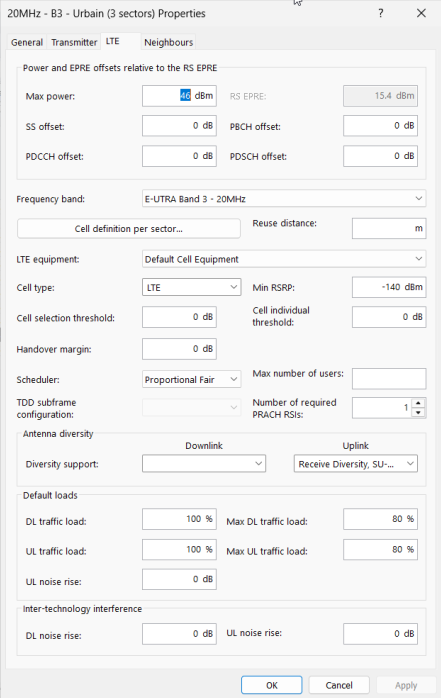
\includegraphics[width=\textwidth]{template_lte.png}\caption{Modèle de station : bande 3, \SI{20}{\mega\hertz}, \SI{46}{\dBm}.}\end{subfigure}\hfill
\begin{subfigure}[b]{0.66\textwidth}\centering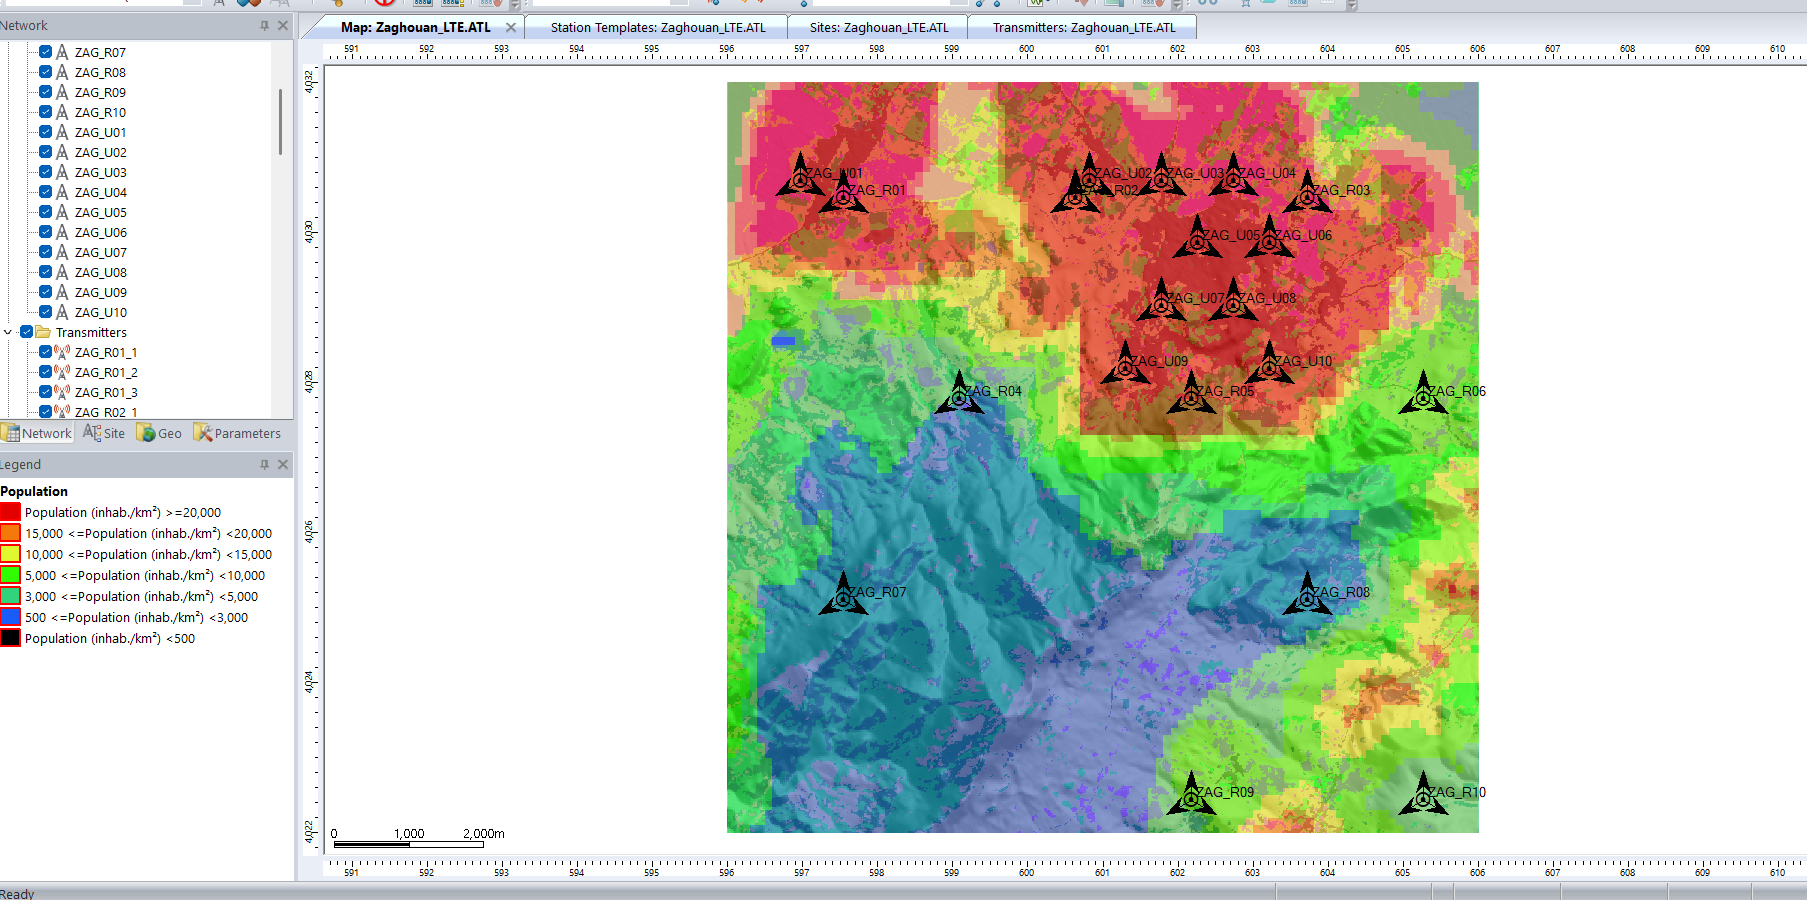
\includegraphics[width=\textwidth]{S02-05_reseau_complet.png}\caption{Le réseau initial : 20 sites, 60 émetteurs.}\end{subfigure}
\caption{Le réseau de l'Étape 1 construit dans Atoll.}
\label{fig-atoll-reseau}
\end{figure}

\section{Le réseau initial}

Les 20 sites du plan nominal (\cref{sec-nominal}) ont été collés dans la table des sites depuis le fichier de coordonnées produit par l'Étape 1 ; Atoll a lu leurs altitudes sur le MNT, cohérentes avec les nôtres. Chaque site a reçu une station de trois secteurs, d'azimuts \ang{0}, \ang{120} et \ang{240}, soit \textbf{60 émetteurs}. Le critère de couverture est un seuil unique sur le niveau du signal de référence (RSRP), déduit du même bilan de liaison. Atoll ajoute lui-même, par classe, l'effet de masque et la pénétration indoor ; le seuil ne doit donc contenir que la marge d'interférence. L'affaiblissement limite en UL vaut alors $P_{\text{UE}} + G - L - S - M_{\text{interf}}$, et le RSRP reçu à cet affaiblissement vaut $\text{RS EPRE} + G - L$ moins cet affaiblissement. Les gains d'antenne s'annulent :
\begin{equation}
  \text{RSRP}_{\min} = \text{RS EPRE} - P_{\text{UE}} + S + M_{\text{interf}} = 15{,}2 - 23 - 114{,}4 + 2 \approx \SI{-120}{\dBm}.
\end{equation}

\section{Le trafic}

Le trafic des simulations Monte-Carlo suit la population : une carte de densité d'utilisateurs a été créée à partir de notre carte de population (\enquote{1 habitant = 1 utilisateur potentiel}), avec tous les utilisateurs actifs en UL et en DL. Chaque simulation applique ensuite un facteur d'échelle qui fixe le nombre d'utilisateurs tirés. Le mélange de services, de mobilités et de terminaux est une hypothèse de travail :

\begin{table}[H]
\centering
\caption{Paramètres de trafic des simulations Monte-Carlo.}
\label{tab-mix}
\begin{tabularx}{\textwidth}{@{}lL@{}}
\toprule
\thead{Paramètre} & \thead{Valeur} \\
\midrule
Services & High Speed Internet \SI{60}{\percent}, Mobile Internet Access \SI{25}{\percent}, VoIP \SI{15}{\percent} \\
Mobilités & piéton \SI{70}{\percent}, \SI{50}{\kilo\metre\per\hour} \SI{20}{\percent}, fixe \SI{10}{\percent} \\
Terminal & MIMO 2 × 2 (\SI{100}{\percent}) \\
Part d'utilisateurs à l'intérieur & \SI{70}{\percent} dans le bâti, \SI{0}{\percent} ailleurs \\
\bottomrule
\end{tabularx}
\end{table}

\begin{retenir}
Le réseau d'Atoll est exactement celui de l'Étape 1 : mêmes 20 sites, même modèle Hata, même puissance, mêmes antennes, mêmes marges. La seule différence voulue est la diffraction sur le relief réel.
\end{retenir}
